%Reference: http://multimediaeval.pbworks.com/w/page/79427054/WorkingNotesPaper2014
\documentclass{acm_proc_article-me}  

\usepackage{color}
\usepackage{graphicx}
\usepackage{booktabs}
\usepackage{url}
\usepackage{caption}
\usepackage{subcaption}
\usepackage{textcomp}
\usepackage{multirow}
\usepackage{blindtext}
\usepackage{algorithm}
\usepackage[noend]{algpseudocode}

%Package to balance last page of two-column layout
%\usepackage{flushend}

\hyphenation{Media-Eval}

\begin{document}

\title{TUW @ Retrieving Diverse Social Images Task 2014}
%\subtitle{[Extended Abstract]
%\titlenote{A full version of this paper is available as

\conferenceinfo{\textit{MediaEval 2014 Workshop,}}{October 16-17, 2014, Barcelona, Spain} 

\numberofauthors{4}
\author{
\alignauthor
Jo\~{a}o R. M. Palotti\\
\affaddr{Vienna University of Technology}\\
%       \affaddr{Favoritenstrasse 9-11/188, 1040 Vienna, Austria}\\
%       \affaddr{Austria}\\
       \email{palotti@ifs.tuwien.ac.at}
\alignauthor
Navid Rekabsaz\\
       \affaddr{Vienna University of Technology}\\
%       \affaddr{Austria}\\
       \email{rekabsaz@ifs.tuwien.ac.at}
\and
\alignauthor
Mihai Lupu\\
       \affaddr{Vienna University of Technology}\\
%       \affaddr{Austria}\\
       \email{lupu@ifs.tuwien.ac.at}
\alignauthor
Allan Hanbury\\
       \affaddr{Vienna University of Technology}\\
       \email{hanbury@ifs.tuwien.ac.at}
}

%OR:
%\numberofauthors{1} 
%\author{\alignauthor Jo\~ao R. M. Palotti, Navid Rekabsaz, Mihai Lupu, and Allan Hanbury\\
%\affaddr{Vienna University of Technology} \\ %%% \affaddr{ Vienna, Austria} \\
%\affaddr{Favoritenstrasse 9-11/188, 1040 Vienna, Austria}\\
%\email{palotti,rekabsz, lupu, hanbury  @ifs.tuwien.ac.at}
%}

%\numberofauthors{1}
%\author{
%\alignauthor
%Jo\~ao R. M. Palotti, Navid Rekabsaz, Mihai Lupu, Allan Hanbury\\
%\affaddr{Vienna University of Technology}\\
%\email{\{palotti, rekabsz, lupu, hanbury\}@ifs.tuwien.ac.at}
%}

\newcommand\todo[1]{\textcolor{red}{[#1]}}
%uncomment to remove all todos:
%\newcommand\todo[1]{}

\maketitle

\begin{abstract}
This paper describes the efforts of Vienna University of Technology (TUW) in the MediaEval 2014 Retrieving Diverse Social Images challenge.
Our approach consisted of 3 steps: (1) a pre-filtering based on Machine Learning, (2) a re-ranking based on Word2Vec, and (3) a clustering part based on an ensemble of clusters. 
Our best run reached a F@20 of 0.564. 

\end{abstract}

%%%%%%%%%%%%%%%%%%%%%%%%%%%%%%%% INTRODUCTION %%%%%%%%%%%%%%%%%%%%%%%%%%%%%%%%%%%%%%%
\begin{section}{Introduction}

Diversification is an interesting problem for the information retrieval community, 
being a challenge for both text and multimedia data.
Focused on image retrieval, the MediaEval 2014 Retrieving Diverse Social Images Task \cite{overview14}
was proposed to foster the development and evaluation of methods for retrieving 
diverse images of different point of interest.

%These tables are put here, just because I want them to be in the second page of this report.

\begin{table*}[htb]
%\footnotesize
\centering
\scriptsize
\caption{Each run and its settings.}
\vspace{-0.25cm}
\label{table:config}
\begin{tabular}{c|c|c|c|c}
\toprule 
\textbf{Run} & \textbf{Pre-Filtering} & \textbf{Re-Ranking} & \textbf{Clustering} & \textbf{Credibility}\tabularnewline
\midrule
\textbf{1} & Based on ML & - & Combined on HOG,CN3x3,CN & -\tabularnewline
\textbf{2} & - & Word2Vec & Metis on Text Similarity & -\tabularnewline
\textbf{3} & - & Word2Vec & Combined on HOG,CN3x3,CN & -\tabularnewline
\textbf{4} & - & Word2Vec & Combined on HOG,CN3x3,CN & ML to remove elements\tabularnewline
\textbf{5} & Based on ML & Word2Vec & Combined on HOG,CN3x3,CN & ML to re-rank elements\tabularnewline
\bottomrule 
\vspace{-0.25cm}
\end{tabular}
\end{table*}




\begin{table*}[hbt]
%\footnotesize
\scriptsize
\centering
\begin{tabular}{c|c|c|c|c|c|c|c|c|c|c|c|c}
\toprule 
\multirow{2}{*}{\textbf{Run}} & \multicolumn{6}{c|}{\textbf{2014 Development Set}} & \multicolumn{6}{c}{\textbf{2014 Test Set}}\tabularnewline
\cmidrule{2-13} 
 & \textbf{P@10} & \textbf{CR@10} & \textbf{F1@10} & \textbf{P@20} & \textbf{CR@20} & \textbf{F@20} & \textbf{P@10} & \textbf{CR@10} & \textbf{F1@10} & \textbf{P@20} & \textbf{CR@20} & \textbf{F@20}\tabularnewline
\midrule
\textbf{1} & 0.830 & 0.294 & 0,431 & 0.778 & 0.477 & 0.588 & 0.796 & 0.284  & 0.414  & 0.748  & 0.462  & 0.564\tabularnewline
\textbf{2} & 0.903 & 0.262 & 0.400 & 0.870 & 0.425 & 0.564 & 0.806 & 0.251  & 0.377  & 0.773  & 0.381  & 0.501\tabularnewline
\textbf{3} & 0.870 & 0.301 & 0.444 & 0.813 & 0.483 & 0.601 & 0.794 & 0.281  & 0.410  & 0.744  & 0.449  & 0.553\tabularnewline
\textbf{4} & 0.890 & 0.297 & 0.441 & 0.827 & 0.503 & 0.619 & 0.806 & 0.280 & 0.412 & 0.754  & 0.443 &  0.552\tabularnewline
\textbf{5} & 0.837 & 0.299 & 0.435 & 0.792 & 0.478 & 0.588 & 0.780 & 0.276 & 0.403 & 0.729 & 0.444 &  0.546\tabularnewline
\bottomrule 
\end{tabular}
\caption{All results - best run according to the official metric was Run1 reaching a F@20 of 0.564}
\label{table:results}
\end{table*}



\end{section}

%%%%%%%%%%%%%%%%%%%%%%%%%%%%%%%% INTRODUCTION %%%%%%%%%%%%%%%%%%%%%%%%%%%%%%%%%%%%%%%

\begin{section}{Methods}
We employed a distinct set of methods for each run. 
Here we explain all the approaches and in Table~\ref{table:config} we show the combinations used for each run.

\begin{subsection}{Pre-Filtering}
We employed a pre-filtering step to exclude likely irrelevant pictures.
%For the 2014 development set, we calculated that 70\% (6256) were relevant images, while 30\% (2667) were not.
The goal of this step is to increase the percentage of relevant images.
We studied two approaches: (1) a filtering step based on a simplified version of Jain et al.~\cite{wsp13} experiments, removing images without any view, geotagged more than 8 kilometers away from the point of interest (POI) and with a description length longer than 2000 characters; 
%(2) apart of these three features, we also used the images' license, the part of the day (morning, afternoon, night) and the number of times the POI appeared 
%in the title and descriptions of an image, and used a Logistic Regression classifier trained on the whole 2013 and 2014 development data.
(2) we trainied a Logistic Regression classifier on the whole 2013 and 2014 development data, using as features the three features described and also the images' license, the part of the day (morning, afternoon, night) and the number of times the POI appeared in the title and descriptions of an image.
\end{subsection}


\begin{subsection}{Re-ranking}

For re-ordering the results, we used the title, tags and description of the photos. For text pre-processing, we de-compounded the terms using a greedy dictionary based approach. In the next step, we expand the query using the first sentence of Wikipedia which helped for place disambiguation. We tested four document similarity methods based on Solr\footnote{http://lucene.apache.org/solr/}, Random Indexing\footnote{https://code.google.com/p/semanticvectors/}, Galago\footnote{http://sourceforge.net/p/lemur/galago/} and Word2Vec\footnote{https://code.google.com/p/word2vec/}\cite{word2vec}. Among all, we found the best result using a semantic similarity approach based on Word2Vec.

Word2Vec provides vector representation of words by using deep learning. We trained a model on Wikipedia and then used the vector representation of words to calculate the text similarity of the query to each photo.

We extracted binary attributes based on Jain et al.~\cite{wsp13}, as we also did in the pre-filtering step, and together with the Word2Vec scores, we used a Linear Regression to re-rank the results based on the development data.


%: (1) if the photo had any view, (2) if the distance between a photo and the POI is greater than 8 kilometers, and (3) if the description length has more than 2000 characters. All features were applied in a Linear Regression model in order to re-rank the list.

\end{subsection}


\begin{subsection}{Clustering}

We worked on three methods for clustering, all based on similarity measures.
%They share the idea of creating a similarity graph $G$ (potentially complete) in which each vertice $V$ represents an images for one point of interest, and
%each edge $E$ represents the similarity between two images accoring to a similarity metric $M$ based on a set of features $F$.
They share the idea of creating a similarity graph (potentially complete) in which each vertex represents an image for one point of interest, and
each edge represents the similarity between two images. Different similarity metrics and different set of features can be used.
%Figure~\ref{fig:bigben} shows a small sample based on 4 images of Big Ben.
Next, we explain each algorithm and how we combined them.

%\begin{figure}[h!]
%\centering
%\includegraphics[width=0.3\textwidth]{figs/bigben}
%\caption{This figure is terrible...I will improve it soon}
%\label{fig:bigben}
%\end{figure}

\begin{subsubsection}{Metis}

%The best way for partitioning $G$ is NP-hard...
The first approach, called Metis \cite{metis},
tries to collapse similar and neighbor vertices, reducing the initial graph to a smaller one (known as coarsening step).
Then, it divides the coarsest graph into a pre-defined number of graphs, generating the clusters.  

\end{subsubsection}

\begin{subsubsection}{Spectral}

Spectral clustering \cite{spectral} can also be seen as a graph partitioning method, which measures both the total dissimilarity between groups 
as well as the total similarity within a group. We used the 
Scikit-learn\footnote{http://scikit-learn.org/} 
%Scikit-learn\footnote{http://scikit-learn.org/stable/modules/generated/sklearn.cluster.SpectralClustering.html} 
implementation of this method. 


\end{subsubsection}

\begin{subsubsection}{Hierarchical}
Hierarchical clustering \cite{hierarchical} is based on the idea of a hierarchy of clusters. A tree is built in a way that the root gathers all the samples and the leaves are clusters with only one sample. This tree can be built bottom-up or top-down. We used the bottom-up implementation from 
%Scikit-learn\footnote{http://scikit-learn.org/stable/modules/generated/sklearn.cluster.AgglomerativeClustering.html}}.
Scikit-learn.

\end{subsubsection}

\begin{subsubsection}{Merging}

%After applying different clustering methods on the whole 2013 and 2014 development set, 
We found that the clustering methods were unstable as modifications in the filtering step caused a great variation in the clustering step.
Therefore, we decided to implement a merging heuristic, which takes into account different points of view from each clustering method and/or feature set,
being potentially more robust than using one single algorithm.

%First, we run each clustering algorithm using a different feature set (for example, HOG, CN, and text similarity) and a different distance measure (in our experiments we used both cosine and Chebyshev) for each POI. It generates a large number of possible cluster results (according to the numbers in this example: 3 algorithms $\times$ 3 feature sets $\times$ 2 measures $=$ 18 possible ways to make clusters). 
%We then created a re-ranking heuristic based only on the frequency that two documents occur in the same cluster.

%%%%
%Each clustering algorithm takes a feature set and a distance measure and outputs a possible way to cluster the images of a POI.
%%%%

Given $c$ different clustering algorithms, $f$ different feature sets, and $m$ distance measures, there are $c \times f \times m$ possible cluster sets. 
In our work, we used the 3 algorithms described, 3 features sets (HOG, CN, CN3x3, see \cite{overview14} for details about these features) and 2 distance measures (cosine and Chebyshev), giving us 18 different cluster sets for each POI.
We can then compute a \emph{frequency matrix} that will hold for every two documents the number of cluster sets in which they occur in the same cluster.
Next we create a re-ranked list of the images from the original list (Flickr ranking) based only on this frequency matrix.
In order to do that, we define a threshold $t$ and a function $F$ on a set of frequencies that determine when a document should be moved to the re-ranked list.
Suppose the re-ranked list contains the documents $D_1, ..., D_i$ and we want to know if a document $D_k$ in the original list can be moved to the re-ranked list at position $i+1$. We compute the frequencies $f_1, ..., f_i$ between $D_k$ and each $D_1,...,D_i$ and if $F(f_1, ..., f_i) < t$, $D_k$ is moved to the re-ranked list, otherwise it is not. 
After all the elements in the original list are processed, if there are still remaining documents not moved to the re-ranked list, the value of $t$ is increased and these documents are reprocessed. The algorithm continues until there are no documents left in the original list.
The functions for $F$ used in this work were maximum, minimum and mean, but other measures, such as mode, median or any percentile could be easily employed as well.

%We start the procedure moving one pivot document (in this work, the top ranked document in the original list) to the re-ranked list. 
%Then, for each document $D_i$ from the original list, we count the number of times that $D_i$ occurred together with each element in the re-ranked list. 
%If any of these frequency values is bigger than a pre-defined $Max\_Threshold$ (6 out of 18, for example), we do not move $D_i$ to the re-ranked list, because $D_i$ co-occurred frequently with another document that is already in the re-ranked list. However, if $D_i$ was not frequently seen with any other document, then we move $D_i$ from the original list to the end of the re-ranked list.
%After trying to move all the documents from the original list to the re-ranked list, we increase the $Max\_Threshold$ to allow more documents in the re-ranked list.
%, so we can accept an image even that a greater number of clustering methods assign that image to the same cluster of another image.
%Usually this is the case of the least ranked elements.
%The algorithm stops when all documents are moved from the original list to the re-ranked one.
%After testing all the elements from the original list, we can start over again from the first document in the original list not yet moved to the re-ranked list, but this time accepting any document that is not see $Max\_Threshold + Max\_increment$. Once all documents were moved from the original list to the re-ranked list, the procedure ends.
%testing all the elements from the original list, we can start over again from the first document in the original list not yet moved to the re-ranked list, but this time accepting any document that is not see $Max\_Threshold + Max\_increment$. Once all documents were moved from the original list to the re-ranked list, the procedure ends.
%We also use a $Min\_Threshold$ and a $Mean\_Threshold$, but other measures, such as the median or any percentile could be easily employed as well.

%Algorithm~\ref{alg:merge} shows the algorithm in more details.
%\renewcommand{\algorithmicrequire}{\textbf{Input:}}
%\renewcommand{\algorithmicensure}{\textbf{Output:}}
%\newcommand{\algorithmicbreak}{\textbf{break}}
%\newcommand{\Break}{\State \algorithmicbreak}
%\algrenewcommand\Return{\State \algorithmicreturn{} }%
%\begin{algorithm}
%\caption{Merging of different clustering methods}
%\label{alg:merge}
%\begin{algorithmic}[1]
%\Require L, F, min, mean, max, min\_increment, mean\_increment, max\_increment
%\Ensure FinalList 

%\Procedure{Merge}{}
%\State $\text{FinalList} \gets \text{[ ]}$
%\State $\textit{pivot} \gets \text{L.pop()}$
%\State $\text{finalList.push(pivot)}$
%\While{L.hasElement()}
%\State $\textit{e} \gets \text{L.pop()}$
%\State $\text{include} \gets \text{True}$

%\State $\text{TempList} \gets \text{[ ]}$
%\ForAll {Element $ie$ in finalList}
%\State $\text{TempList} \gets \text{F[e][ie]}$
%\EndFor

%\If {max(TempList) > maxvalue} 
%\State $\text{include} \gets \text{False}$
%\Break
%\EndIf
%\If {min(TempList) > minvalue} 
%\State $\text{include} \gets \text{False}$
%\Break
%\EndIf
%\If {mean(TempList) > meanvalue} 
%\State $\text{include} \gets \text{False}$
%\Break
%\EndIf
%\If {include} 
%\State $\text{finalList.push(ie)}$
%\Else
%\State $\text{L.push(ie)}$
%\EndIf
%\State $\text{min} \gets \text{min} + \text{min\_increment}$
%\State $\text{max} \gets \text{max} + \text{max\_increment}$
%\State $\text{mean} \gets \text{mean} + \text{mean\_increment}$
%\EndWhile
%\Return finalList
%\EndProcedure
%\end{algorithmic}
%\end{algorithm}

\end{subsubsection}

\end{subsection}

\begin{subsection}{Credibility}
%The credibility data was not available for 2013, therefore the amount of data was relatively small. 
%Even so, 
Our approaches were based on Machine Learning (ML): we trained a Logistic Regression classifier to learn if a document was relevant or not based on the credibility data (used only face proportion, location similarity, upload frequency and bulk proportion).
We tested two methods: (1) excluding documents set as irrelevant for Run4 and (2) moving to the bottom of the list irrelevant documents for Run5.

\end{subsection}
\end{section}

\begin{section}{Experiments}

We submitted all 5 runs, varying on the use of pre-filtering, the re-ranking method, the clustering approach and the use of credibility.
Details are shown in Table~\ref{table:config} and the results are shown in Table~\ref{table:results}.
Based on the development data, we were expecting Run3 and Run4 to be our best runs, but the results on the test data shows that we probably 
overfitted the development set for the re-ranking and credibility part. The best result was that the cluster ensemble proved to be robust for this task.

% Moved to introduction, so the tables can be placed in the second page
%
\begin{table*}[htb]
%\footnotesize
\centering
\scriptsize
\caption{Each run and its settings.}
\vspace{-0.25cm}
\label{table:config}
\begin{tabular}{c|c|c|c|c}
\toprule 
\textbf{Run} & \textbf{Pre-Filtering} & \textbf{Re-Ranking} & \textbf{Clustering} & \textbf{Credibility}\tabularnewline
\midrule
\textbf{1} & Based on ML & - & Combined on HOG,CN3x3,CN & -\tabularnewline
\textbf{2} & - & Word2Vec & Metis on Text Similarity & -\tabularnewline
\textbf{3} & - & Word2Vec & Combined on HOG,CN3x3,CN & -\tabularnewline
\textbf{4} & - & Word2Vec & Combined on HOG,CN3x3,CN & ML to remove elements\tabularnewline
\textbf{5} & Based on ML & Word2Vec & Combined on HOG,CN3x3,CN & ML to re-rank elements\tabularnewline
\bottomrule 
\vspace{-0.25cm}
\end{tabular}
\end{table*}



%
\begin{table*}[hbt]
%\footnotesize
\scriptsize
\centering
\begin{tabular}{c|c|c|c|c|c|c|c|c|c|c|c|c}
\toprule 
\multirow{2}{*}{\textbf{Run}} & \multicolumn{6}{c|}{\textbf{2014 Development Set}} & \multicolumn{6}{c}{\textbf{2014 Test Set}}\tabularnewline
\cmidrule{2-13} 
 & \textbf{P@10} & \textbf{CR@10} & \textbf{F1@10} & \textbf{P@20} & \textbf{CR@20} & \textbf{F@20} & \textbf{P@10} & \textbf{CR@10} & \textbf{F1@10} & \textbf{P@20} & \textbf{CR@20} & \textbf{F@20}\tabularnewline
\midrule
\textbf{1} & 0.830 & 0.294 & 0,431 & 0.778 & 0.477 & 0.588 & 0.796 & 0.284  & 0.414  & 0.748  & 0.462  & 0.564\tabularnewline
\textbf{2} & 0.903 & 0.262 & 0.400 & 0.870 & 0.425 & 0.564 & 0.806 & 0.251  & 0.377  & 0.773  & 0.381  & 0.501\tabularnewline
\textbf{3} & 0.870 & 0.301 & 0.444 & 0.813 & 0.483 & 0.601 & 0.794 & 0.281  & 0.410  & 0.744  & 0.449  & 0.553\tabularnewline
\textbf{4} & 0.890 & 0.297 & 0.441 & 0.827 & 0.503 & 0.619 & 0.806 & 0.280 & 0.412 & 0.754  & 0.443 &  0.552\tabularnewline
\textbf{5} & 0.837 & 0.299 & 0.435 & 0.792 & 0.478 & 0.588 & 0.780 & 0.276 & 0.403 & 0.729 & 0.444 &  0.546\tabularnewline
\bottomrule 
\end{tabular}
\caption{All results - best run according to the official metric was Run1 reaching a F@20 of 0.564}
\label{table:results}
\end{table*}



\end{section}
\begin{section}{Conclusion}

Our experiments show that an ensemble of clusters can be a robust way to diversify results.
Unfortunately our re-rank method did not work in the test set as well as it did in the development set.
Last, the use of credibility also seems to have overfitted the development data, not being effective for the test set.

\end{section}

\paragraph{\textbf{ACKNOWLEDGMENTS}}
%\begin{section}{ACKNOWLEDGMENTS}
This research was funded by the Austrian Science Fund (FWF) project number I1094-N23 (MUCKE) and project number P25905-N23 (ADmIRE). 
%\end{section}

\bibliographystyle{abbrv}
\bibliography{workingNotes}  
\end{document}
